\documentclass[a4paper]{article}
\usepackage{cmap}
\usepackage[utf8]{inputenc}
\usepackage[T2A]{fontenc}
\usepackage[english,russian]{babel} 
\usepackage[left=15mm, top=15mm, right=15mm, bottom=30mm, nohead, nofoot]{geometry}
\usepackage{blindtext}  % рыба-текст
\usepackage{graphicx}  % изобржаения
\usepackage{float} % плавающие объекты
\usepackage{wrapfig}  % изобржаения
\usepackage{tikz} % графика
\usepackage{mdframed} % рамки
\usepackage{xcolor} % определение цветов
\usepackage{nicefrac} % красивые дроби
\usepackage{cancel} % сокращение
\usepackage{amsmath,amsfonts,amssymb} % математический пакет
\usepackage{hyperref}  % гиперссылки
\usepackage{fancybox,fancyhdr} % хедер и футер
\usepackage{listings} % код
\usepackage[skip=2pt]{caption} % расстояние между подписью и картинкой
\pagestyle{fancy}
\fancyhf{}
\fancyhead[L]{Лабораторная работа №5}
\fancyhead[R]{\textit{Связь непрерывного и дискретного}}
\fancyfoot[C]{\thepage}
\headsep=4mm
\footskip=13mm
\setlength{\parindent}{0em}
\setlength{\parsep}{0em}
\setlength{\headheight}{12pt}
\setlength{\topmargin}{-38pt}

\definecolor{urlcolor}{HTML}{3454D1}
\definecolor{linkcolor}{HTML}{3454D1}
\hypersetup{
    pdfstartview=FitH,
    linkcolor=linkcolor,
    urlcolor=urlcolor,
    colorlinks=true,
    pdftitle={Лабораторная работа №5},
    pdfauthor={Овчинников П.А.}
}

\definecolor{strings}{rgb}{0,0.6,0}
\definecolor{comments}{rgb}{0,0.3,0}
\definecolor{numbers}{rgb}{0.5,0.5,0.5}
\definecolor{keywords}{rgb}{0.09,0.61,0.95}
\definecolor{background}{rgb}{0.97,0.97,0.97}
\lstdefinestyle{codestyle}{
    backgroundcolor=\color{background},
    commentstyle=\color{comments},
    keywordstyle=\color{keywords},
    stringstyle=\color{strings},
    numberstyle=\tiny\color{numbers},
    basicstyle=\ttfamily\footnotesize,
    breakatwhitespace=false,
    breaklines=true,
    captionpos=b,
    inputencoding=utf8,
    keepspaces=true,
    numbers=left,
    numbersep=5pt,
    showspaces=false,
    showstringspaces=false,
    showtabs=false,
    tabsize=2,
    extendedchars=true,
    literate=
    {а}{{\cyra}}1
    {б}{{\cyrb}}1
    {в}{{\cyrv}}1
    {г}{{\cyrg}}1
    {д}{{\cyrd}}1
    {е}{{\cyre}}1
    {ж}{{\cyrzh}}1
    {з}{{\cyrz}}1
    {и}{{\cyri}}1
    {й}{{\cyrishrt}}1
    {к}{{\cyrk}}1
    {л}{{\cyrl}}1
    {м}{{\cyrm}}1
    {н}{{\cyrn}}1
    {о}{{\cyro}}1
    {п}{{\cyrp}}1
    {р}{{\cyrr}}1
    {с}{{\cyrs}}1
    {т}{{\cyrt}}1
    {у}{{\cyru}}1
    {ф}{{\cyrf}}1
    {х}{{\cyrh}}1
    {ц}{{\cyrc}}1
    {ч}{{\cyrch}}1
    {ш}{{\cyrsh}}1
    {щ}{{\cyrshch}}1
    {ъ}{{\cyrhrdsn}}1
    {ы}{{\cyrery}}1
    {ь}{{\cyrsftsn}}1
    {э}{{\cyrerev}}1
    {ю}{{\cyryu}}1
    {я}{{\cyrya}}1
    {А}{{\CYRA}}1
    {Б}{{\CYRB}}1
    {В}{{\CYRV}}1
    {Г}{{\CYRG}}1
    {Д}{{\CYR96}}1
    {Е}{{\CYRE}}1
    {Ж}{{\CYRZH}}1
    {З}{{\CYRZ}}1
    {И}{{\CYRI}}1
    {Й}{{\CYRISHRT}}1
    {К}{{\CYRK}}1
    {Л}{{\CYRL}}1
    {М}{{\CYRM}}1
    {Н}{{\CYRN}}1
    {О}{{\CYRO}}1
    {П}{{\CYRP}}1
    {Р}{{\CYRR}}1
    {С}{{\CYRS}}1
    {Т}{{\CYRT}}1
    {У}{{\CYRU}}1
    {Ф}{{\CYRF}}1
    {Х}{{\CYRH}}1
    {Ц}{{\CYRC}}1
    {Ч}{{\CYRCH}}1
    {Ш}{{\CYRSH}}1
    {Щ}{{\CYRSHCH}}1
    {Ъ}{{\CYRHRDSN}}1
    {Ы}{{\CYRERY}}1
    {Ь}{{\CYRSFTSN}}1
    {Э}{{\CYREREV}}1
    {Ю}{{\CYRYU}}1
    {Я}{{\CYRYA}}1
}
\lstset{style=codestyle}

\addto\captionsrussian{
  \renewcommand{\contentsname}
    {\centering Содержание}
}
\newcommand{\addsection}[1]{
    \phantomsection
    \addcontentsline{toc}{section}{#1}
    \section*{\centering #1}
}
\newcommand{\addsubsection}[1]{
    \phantomsection
    \addcontentsline{toc}{subsection}{#1}
    \subsection*{\centering #1}
}
\newcommand{\addsubsubsection}[1]{
    \phantomsection
    \addcontentsline{toc}{subsubsection}{#1}
    \subsubsection*{\centering #1}
}

\newmdenv[
    leftmargin = 0.5em,
    skipabove = 0.5em,
    skipbelow = 0.5em,
    linewidth = 1pt,
    rightline = false,
    topline = false,
    bottomline = false
]{quotebox}

\newlength{\tempheight}
\newcommand{\Let}{
\mathbin{\text{\settoheight{\tempheight}{\mathstrut}\raisebox{0.4\pgflinewidth}{
\tikz[baseline=0.5ex,line cap=round,line join=round] \draw (0,0) --++ (0.3em,0) --++ (0,2.3ex) --++ (-0.3em,0);
}}}}
\newcommand*\squared[1]{\tikz[baseline=(char.base)]{
            \node[shape=rectangle,draw,inner sep=4pt] (char) {#1};}}
\newcommand*\msquared[1]{\tikz[baseline=(char.base)]{
            \node[shape=rectangle,draw,inner sep=4pt] (char) {$\displaystyle #1$};}}
\newcommand\argmax[1]{\underset{#1}{\text{argmax}}}
\renewcommand\max[1]{\underset{#1}{\text{max}}}
\newcommand{\at}{\biggr\rvert}
\newcommand{\shiftright}[3]{\makebox[#2][r]{\makebox[#1][l]{#3}}}
\newcommand{\e}{\;\text{e}}
\let\oldint\int
\def\int{\oldint\limits}
\DeclareRobustCommand{\divby}{%
  \mathrel{\vbox{\baselineskip.65ex\lineskiplimit0pt\hbox{.}\hbox{.}\hbox{.}}}%
}

\newcommand\NB{\textbf{N\kern-0.32em\textcolor{red}{B}}}

\begin{document}
\begin{titlepage}
    \begin{center}
        \includegraphics[width=0.18\textwidth]{~/Изображения/itmo_logo.png}\\[10pt]
        Федеральное государственное автономное образовательное учреждение высшего образования \\[6pt]
        САНКТ-ПЕТЕРБУРГСКИЙ НАЦИОНАЛЬНЫЙ ИССЛЕДОВАТЕЛЬСКИЙ УНИВЕРСИТЕТ ИТМО \\[16pt]
        Факультет систем управления и робототехники \vfill
        Лабораторная работа №5 \\[0.5em]
        \textbf{\MakeUppercase{Связь непрерывного и дискретного}}
    \end{center}\vfill
    \begin{flushright}
        Студент: Овчинников П.А.\\
        Поток: ЧАСТ.МЕТ. 1.3 \\[0.5em]
        Преподаватель: Перегудин А.А.\\Пашенко А.В.
    \end{flushright}\vfill
    \begin{center}
        {\small Санкт-Петербург \\ 2024}
    \end{center}
\end{titlepage}
\setcounter{page}{2}
\tableofcontents\newpage
% MARK: №1
\addsection{Непрерывное и дискретное преобразование Фурье}
Рассмотрим уже знакомую нам прямоугольную функцию единичного масштаба:
$$\Pi(t) = \begin{cases}
    1, & |t| \leq \nicefrac{1}{2}, \\
    0, & |t| > \nicefrac{1}{2}.
\end{cases}$$
Сейчас мы опробуем на ней различные варианты Фурье-преобразования и выясним, чем они отличаются между собой, какой быстрее, какой точнее и как совместить достоинства разных подходов вместе.
\addsubsection{Истинный Фурье-образ}
Известно, что истинное Фурье-преобразование прямоугольной функции равно:
$$\hat{\Pi}(v) = \int_{-\infty}^{\infty}\Pi(t)\e^{-2\pi ivt}\,dt = \int_{-\nicefrac{1}{2}}^{\nicefrac{1}{2}}\e^{-2\pi ivt}\,dt = \frac{\e^{-\pi iv} - \e^{\pi iv}}{2\pi i v} = \frac{\sin{\pi v}}{\pi v} = \text{sinc}(v)$$
\begin{figure}[H]
    \begin{minipage}{0.49\textwidth}
        \centering 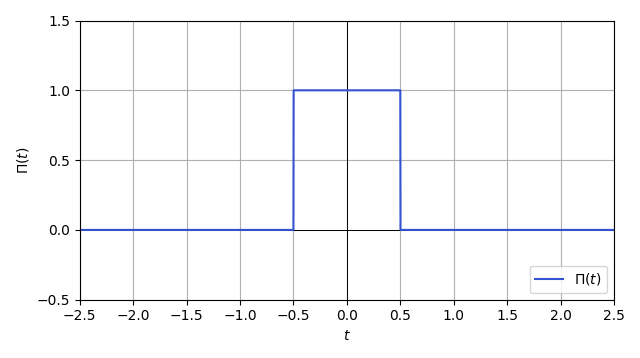
\includegraphics[width=\textwidth]{sources/first/1_square_wave.png}
        \caption{График функции $\Pi(t)$}
    \end{minipage}\hfill
    \begin{minipage}{0.49\textwidth}
        \centering 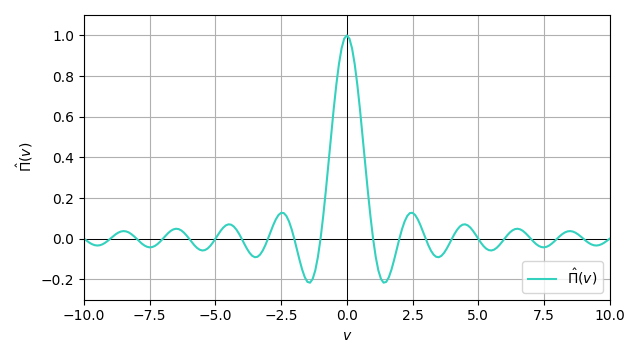
\includegraphics[width=\textwidth]{sources/first/2_true_image.png}
        \caption{График истинного Фурье-образа $\hat{\Pi}(v)$}
    \end{minipage}
\end{figure}
\addsubsection{Численное интегрирование}
Для численного интегрирования воспользуемся функцией \texttt{trapz} из библиотеки \texttt{numpy}. Метод подразумевает, что мы интегрируем по ограниченному промежутку и с заданным шагом интегрирования. Начнём с промежутка $T = 20$ и разбиения на $1000$ точек. Вычислим Фурье-образ $\hat{\Pi}_N(v)$ методом численного интегрирования:
\begin{figure}[H]
    \centering 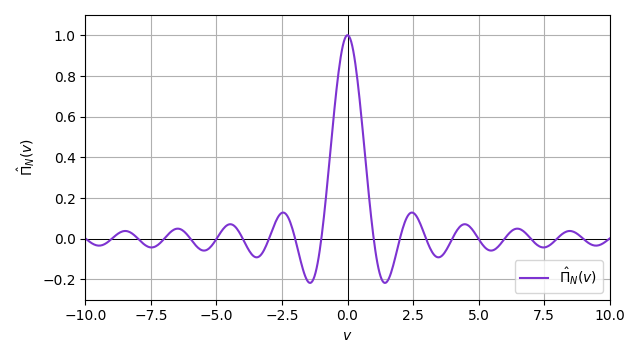
\includegraphics[width=0.6\textwidth]{sources/first/part1/T=20 density=1000/3_num_image.png}
    \caption{График численного Фурье-образа $\hat{\Pi}(v)$ при $T = 20$ и $N = 1000$}
\end{figure}
Как видим, график численного Фурье-образа $\hat{\Pi}_N(v)$ внешне совпадает с истинным Фурье-образом $\hat{\Pi}(v)$, но только внешне.\newpage
Выполним обратное преобразование Фурье и посмотрим на результат:
\begin{figure}[H]
    \centering 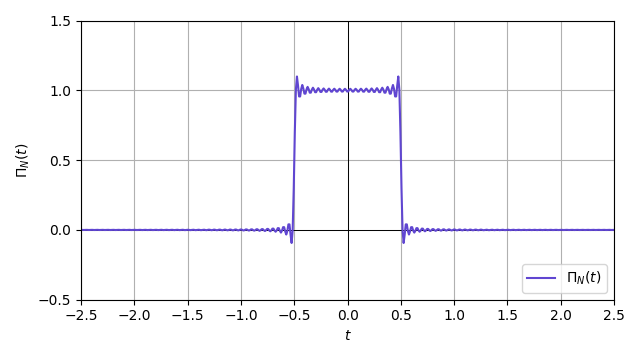
\includegraphics[width=0.6\textwidth]{sources/first/part1/T=20 density=1000/4_num_restored.png}
    \caption{График восстановленной из численного Фурье-образа функции $\Pi_N(t)$ при $T = 20$ и $N = 1000$}
\end{figure}
Возникает эффект Гиббса, который проявляется в виде колебаний вблизи точек разрыва. Это связано с тем, что мы интегрировали по конечному промежутку, а не по всей числовой прямой.Попробуем увеличить промежуток интегрирования до $T = 90$:
\begin{figure}[H]
    \centering 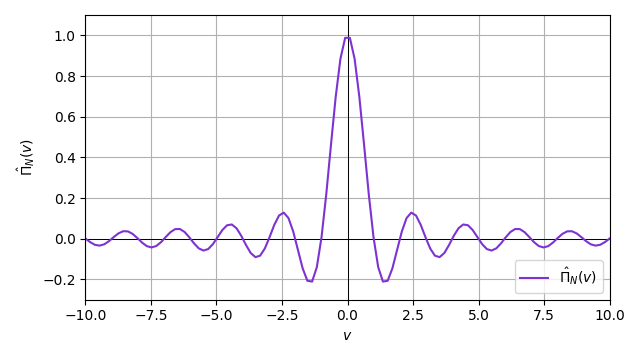
\includegraphics[width=0.6\textwidth]{sources/first/part1/T=90 density=1000/3_num_image.png}
    \caption{График численного Фурье-образа $\hat{\Pi}(v)$ при $T = 90$ и $N = 1000$}
\end{figure}
Промежуток вырос, а то же количество точек равномерно распределилось по большему промежутку --- это понижает точность в вычислении интеграла. На изгибах кардинального синуса наблюдаются неровности.\\[0.5em] Теперь посмотрим на восстановленную функцию:
\begin{figure}[H]
    \centering 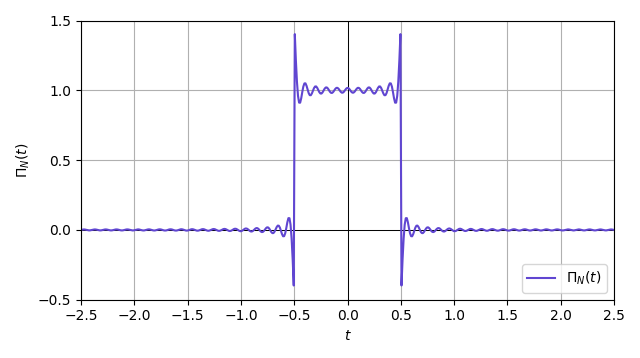
\includegraphics[width=0.6\textwidth]{sources/first/part1/T=90 density=1000/4_num_restored.png}
    \caption{График восстановленной из численного Фурье-образа функции $\Pi_N(t)$ при $T = 90$ и $N = 1000$}
\end{figure}
Ввиду того, что мы увеличили промежуток интегрирования, но не увеличили количество точек, на графике восстановленной функции колебания усилились, ведь гораздо больше высокочастотных гармоник было упущено в образе Фурье.\\[0.5em]
Теперь увеличим количество точек до $N = 10000$:
\begin{figure}[H]
    \centering 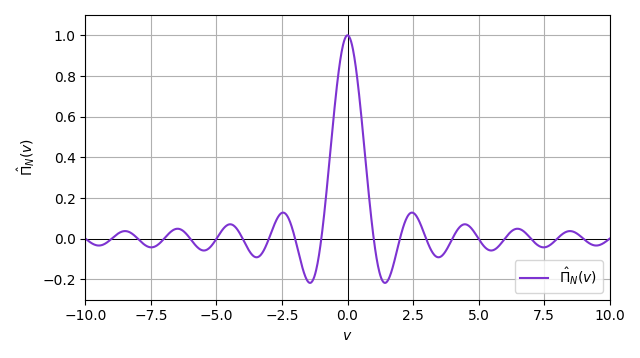
\includegraphics[width=0.6\textwidth]{sources/first/part1/T=90 density=10000/3_num_image.png}
    \caption{График численного Фурье-образа $\hat{\Pi}(v)$ при $T = 90$ и $N = 10000$}
\end{figure}
Кривая образа снова стала гладкой --- вновь восстановим из образа прямоугольную функцию путём обратного преобразования Фурье:
\begin{figure}[H]
    \centering 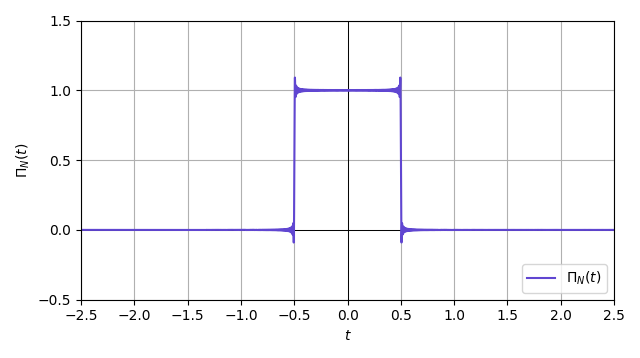
\includegraphics[width=0.6\textwidth]{sources/first/part1/T=90 density=10000/4_num_restored.png}
    \caption{График восстановленной из численного Фурье-образа функции $\Pi_N(t)$ при $T = 90$ и $N = 10000$}
\end{figure}
Амплитуда колебаний на границах разрыва уменьшилась, но они всё равно присутствуют, как ни крути. Что может сказать код на Python о быстродействии такого метода?
\begin{center}
    \begin{minipage}{0.3\textwidth}
        \begin{lstlisting}
trapz #1: 3.07 s
trapz #2: 1.16 s
trapz #3: 19.98 s
\end{lstlisting}
    \end{minipage}
\end{center}
\textbf{Вывод:}
\begin{quotebox}
    Метод \texttt{trapz} работает медленно. При 1000 точек он работает около 2 секунд, а при 10000 точек --- уже 20 секунд. При этом метод достаточно точный, но плохо работает с функциями, имеющими разрывы первого рода.
\end{quotebox} \newpage

\addsubsection{Использование DFT}
Попробуем воспользоваться дискретным преобразованием Фурье. Для этого нам понадобится функция \texttt{fft} из библиотеки \texttt{numpy}. Эта функция реализует быстрое преобразование Фурье, которое математически описывается так:
$$F(k) = \sum_{m=0}^{N - 1}f(m)\exp\left\{ -2\pi i \frac{mk}{N} \right\} \quad\leftrightarrow\quad f(m) = \frac{1}{N}\sum_{k=0}^{N - 1}F(k)\exp\left\{ 2\pi i \frac{mk}{N} \right\}$$
$$F(k) = \frac{1}{\sqrt{N}}\sum_{m=0}^{N - 1}f(m)\exp\left\{ -2\pi i \frac{mk}{N} \right\} \quad\leftrightarrow\quad f(m) = \frac{1}{\sqrt{N}}\sum_{k=0}^{N - 1}F(k)\exp\left\{ 2\pi i \frac{mk}{N} \right\}$$
Чтобы преобразование стало унитарным, нам потребовалось разбить множитель $\nicefrac{1}{N}$ в обратном преобразовании на два $\nicefrac{1}{\sqrt{N}}$ --- это сохранит норму сигнала. В \texttt{numpy.fft} достаточно указать параметр \texttt{norm='ortho'}, чтобы преобразование стало унитарным.\\[0.5em]
Возьмём разбиение на $10000$ точек и проведём преобразование Фурье нашей прямоугольной функции и посмотрим на график образа при таком преобразовании:
\begin{figure}[H]
    \centering 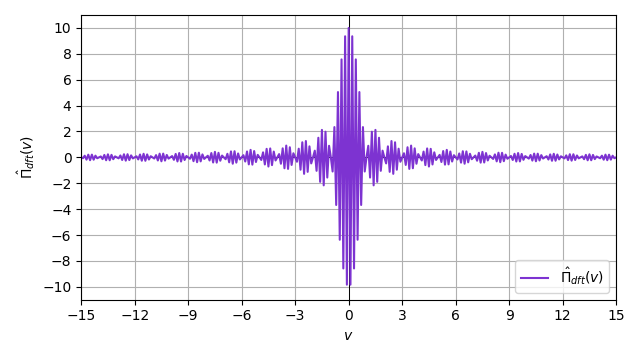
\includegraphics[width=0.55\textwidth]{sources/first/part2/3_dft_image.png}
    \caption{График дискретного Фурье-образа $\hat{\Pi}(v)$}
\end{figure}
Это мало похоже на истинный Фурье-образ. Попробуем восстановить из него прямоугольную функцию:
\begin{figure}[H]
    \centering 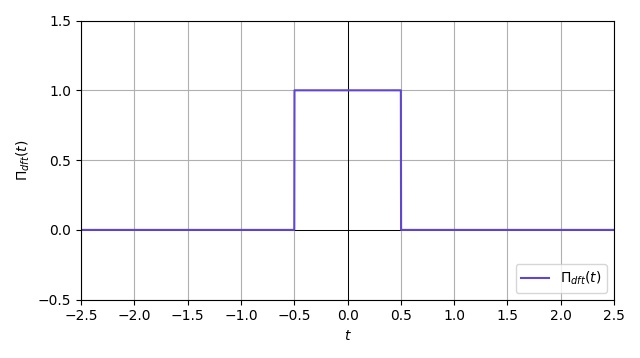
\includegraphics[width=0.55\textwidth]{sources/first/part2/4_dft_restored.png}
    \caption{График восстановленной из дискретного Фурье-образа функции $\Pi_N(t)$}
\end{figure}
Что удивительно, восстановленная функция выглядит ровно так же, как и исходная. При этом код на Python показывает следующие результаты:\vspace{-0.5em}
\begin{center}
    \begin{minipage}{0.3\textwidth}
        \begin{lstlisting}
dft: 0.64 s
\end{lstlisting}
    \end{minipage}
\end{center} \vspace{-0.5em}
\textbf{Вывод:}
\begin{quotebox}
    Метод \texttt{DFT} работает быстро и точно. При 10000 точек он работает около 1 секунды. Это более чем в 30 раз быстрее, учитывая равное количество точек с третьим испытанием метода \texttt{trapz}. При этом метод хорошо работает с функциями, имеющими разрывы первого рода. Но с Фурье-образом что-то пошло не так.
\end{quotebox}

\addsubsection{Выводы о работе trapz и DFT}
Приблизиться к истинному Фурье-образу смог только метод \texttt{trapz}, но он работает медленно и неустойчив к разрывам. Метод \texttt{numpy.fft} работает быстро и точно, но его образ сильно отличается от истинного. С чем это связано?\\[0.5em]
Как следует из названия, метод \texttt{trapz} аппроксимирует интегрирование, разбивая площадь на маленькие трапеции шириной в dt, площадь которых вычислять проще. Для интегрирования с $N + 1$ равномерно расположенными точками аппроксимация работает так:
$$\int_a^b f(x)\,dx \approx \frac{1}{2}\sum_{n=1}^{N}\left( x_{n+1} - x_n \right)\left( f(x_n) + f(x_{n+1}) \right) = \frac{b - a}{2N}\sum_{n=1}^{N}\left( f(x_n) + f(x_{n+1}) \right),\quad \frac{b - a}{N} \sim \left( x_{n+1} - x_n \right)\sim dt$$
Формула с коэффициентом $\nicefrac{1}{2}$ --- для случаев, когда расстояние между точками не фиксированное. Если оно фиксированное, как в случае с преобразованием Фурье, то используется вторая формула.\\[0.5em]
Метод \texttt{numpy.fft} работает по-другому. Он преобразует сигнал в пространство частот, где каждая гармоника имеет свой вес. При этом важно, чтобы сигнал был периодичен, иначе возникнут артефакты. В нашем случае прямоугольная функция не является периодичной, поэтому и образ Фурье отличается от истинного. Формулы унитарного дискретного преобразования были приведены в предыдущем пункте.

\addsubsection{Приближение непрерывного с помощью DFT}
Попробуем переиграть метод \texttt{numpy.fft} и всё же приблизить истинный Фурье-образ $\hat{\Pi}(v)$ с помощью дискретного преобразования Фурье. Рассмотрим интеграл Фурье-преобразования:
$$F(v) = \frac{1}{\sqrt{2\pi}}\int_{-\infty}^{\infty} f(t)e^{-2\pi ivt}\,dt$$
Аппроксимируем его с помощью суммы Римана --- для этого введём замену $t = m\Delta t + t_0 \Rightarrow dt = \Delta t$:
$$F(v) \approx \frac{1}{\sqrt{N}}\sum_{m=0}^{N - 1}f(m\Delta t + t_0)e^{-2\pi iv(m\Delta t + t_0)}\Delta t = \frac{1}{\sqrt{N}}\Delta te^{-2\pi ivt_0}\sum_{m=0}^{N - 1}f(m\Delta t + t_0)\e^{-2\pi ivm\Delta t}$$
Для частот введём замену $v_k = k\Delta v = \nicefrac{k}{N\Delta t}$, а т.к. $t_0$ и $\Delta t$ постоянные, то введём замену $f[n] = f(n\Delta t + t_0)$:
$$F(v_k) \approx \frac{1}{\sqrt{N}}\Delta te^{-2\pi ivt_0}\sum_{m=0}^{N - 1}f[n]\e^{-2\pi iv_km\Delta t} = \frac{1}{\sqrt{N}}\Delta te^{-2\pi ivt_0}\sum_{m=0}^{N - 1}f[n]\e^{-2\pi i\frac{km}{N}}$$
Как ни странно, мы получаем формулу для дискретного преобразования Фурье, но с домножением на фазовый коэффициент $\Delta t\e^{-2\pi ivt_0}$. Назовём такое преобразование \texttt{cdft}. Проведём его на прямоугольной функции:
\begin{figure}[H]
    \centering 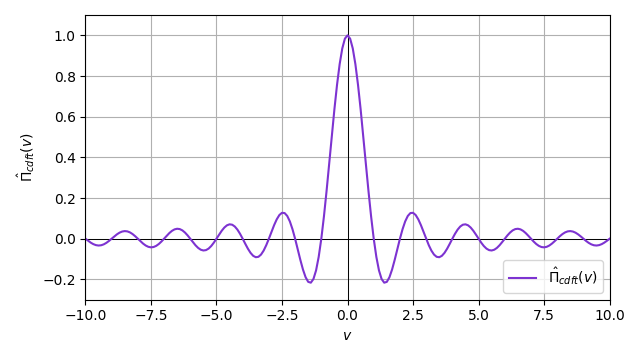
\includegraphics[width=0.55\textwidth]{sources/first/part3/3_dft_continuous_image.png}
    \caption{График приближённого Фурье-образа $\hat{\Pi}_{cdft}(v)$}
\end{figure}
Действительно получаем гладкую кривую, похожую на истинный Фурье-образ. \newpage
Попробуем восстановить из него прямоугольную функцию:
\begin{figure}[H]
    \centering 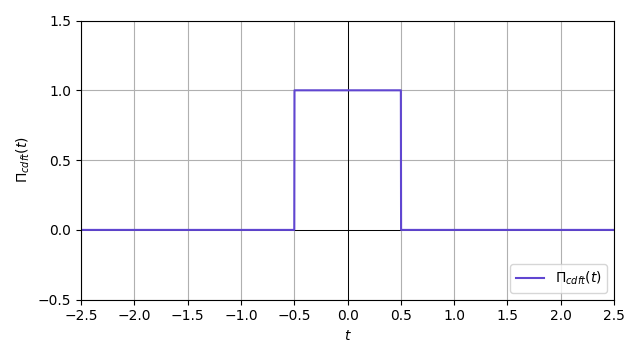
\includegraphics[width=0.55\textwidth]{sources/first/part3/4_dft_continuous_restored.png}
    \caption{График восстановленной из приближённого Фурье-образа функции $\Pi_{cdft}(t)$}
\end{figure}
Восстановленная функция выглядит так же, как и исходная. При этом код на Python показывает следующие результаты:\vspace{-0.5em}
\begin{center}
    \begin{minipage}{0.3\textwidth}
        \begin{lstlisting}
cdft: 0.63 s
\end{lstlisting}
    \end{minipage}
\end{center} \vspace{-0.5em}
\textbf{Вывод:}
\begin{quotebox}
    Проведя некоторые преобразования, мы смогли лишить метод \texttt{DFT} недостатков и приблизить его к истинному Фурье-образу. При этом метод остался быстрым и точным и всё так же отлично работает с функциями, имеющими разрывы первого рода.
\end{quotebox}

% MARK: №2
\addsection{Сэмплирование}
Исследуем теорему Найквиста-Шеннона-Котельникова, которая гласит, что для безошибочного восстановления сигнала из образа, взятого по дискретным данным, на отрезке $[-B, B]$ необходимо, чтобы шаг дискретизации $\Delta t$ подчинялся условию $\Delta t < \nicefrac{1}{(2B)}$. Мы рассмотрим два разных сигнала: сумму двух синусоид и кардинальный синус.\\[0.5em]
Для восстановления сигнала из его дискретного образа будем пользоваться интерполяционной формулой:
$$f(t) = \sum_{n=-\infty}^{\infty}f[n]\,\text{sinc}\left( 2B\left( t-t_n \right) \right),\quad t_n=\frac{n}{2B}$$
\addsubsection{Сэмплирование синусов}
Рассмотрим первую функцию --- сумма синусоид, зададимся параметрами $a_1 = 1$, $\omega_1 = 2$, $\varphi_1 = 3$, $a_2 = 4$, $\omega_2 = 5$, $\varphi_2 = 6$. Так выглядит график функции:
$$y(t) = a_1\sin(\omega_1t + \varphi_1) + a_2\sin(\omega_2t + \varphi_2) = \sin(2t + 3) + 4\sin(5t + 6)$$
\begin{figure}[H]
    \centering 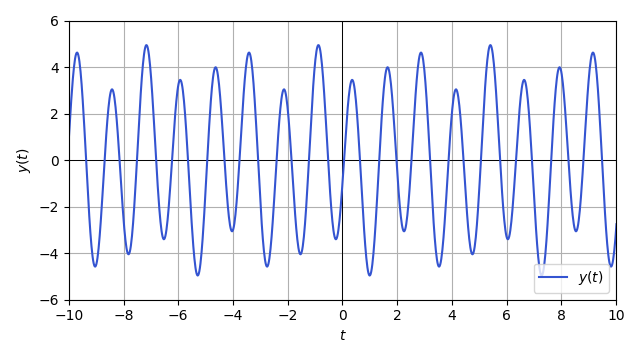
\includegraphics[width=0.52\textwidth]{sources/second/1_sins_y.png}
    \caption{График $y(t)$}
\end{figure}
Теперь проведём сэмплирование сигнала с шагом $\Delta t = \nicefrac{1}{8}$:
\begin{figure}[H]
    \begin{minipage}{0.49\textwidth}
        \centering 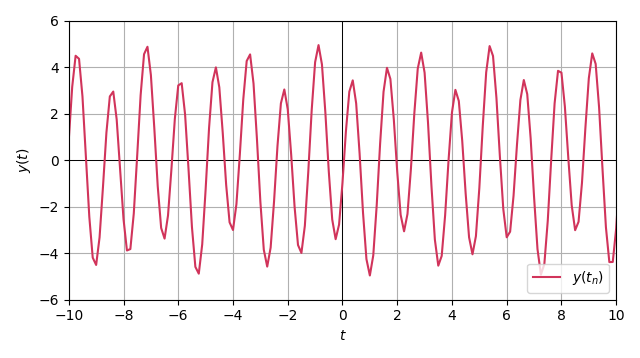
\includegraphics[width=\textwidth]{sources/second/sins dt=0.125 B=4/2_y_sampled.png}
        \caption{График сэмплированного сигнала $y(t_n)$}
    \end{minipage}\hfill
    \begin{minipage}{0.49\textwidth}
        \centering 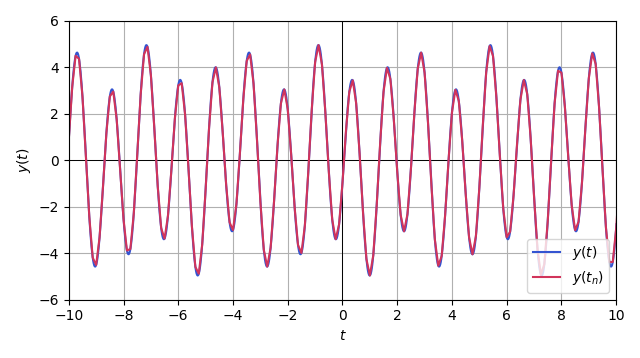
\includegraphics[width=\textwidth]{sources/second/sins dt=0.125 B=4/3_y_cmp(sampling).png}
        \caption{Сравнительный график $y(t)$ и $y(t_n)$}
    \end{minipage}
\end{figure}
На сравнительном графике не сильно заметна разница между сигналами, поэтому слева дополнительно приведён график сэмплированного сигнала отдельно. Теперь попробуем интерполяцией восстановить сигнал по сэмплированному образу с $B = 4$:
\begin{figure}[H]
    \begin{minipage}{0.49\textwidth}
        \centering 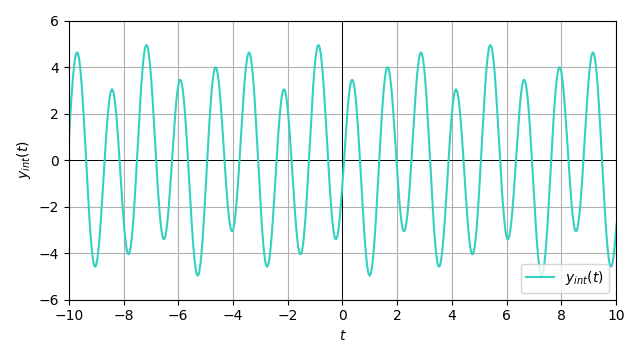
\includegraphics[width=\textwidth]{sources/second/sins dt=0.125 B=4/4_y_interp.png}
        \caption{График восстановленного сигнала $y_{int}(t)$}
    \end{minipage}\hfill
    \begin{minipage}{0.49\textwidth}
        \centering 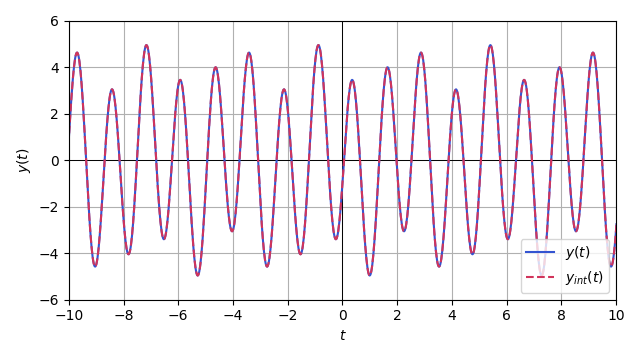
\includegraphics[width=\textwidth]{sources/second/sins dt=0.125 B=4/5_y_cmp(interpolation).png}
        \caption{Сравнительный график $y(t)$ и $y_{int}(t)$}
    \end{minipage}
\end{figure}
Восстановленный сигнал идентичен исходному. Это связано с тем, что $\Delta t = \nicefrac{1}{8} = \nicefrac{1}{(2B)}$.\\[0.5em]
Теперь увеличим шаг сэмплирования до $\Delta t = \nicefrac{1}{4}$:
\begin{figure}[H]
    \begin{minipage}{0.49\textwidth}
        \centering 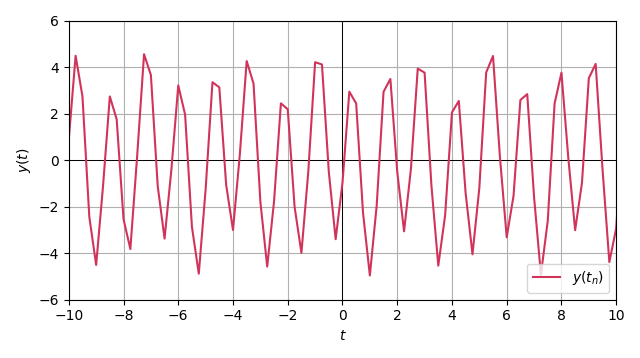
\includegraphics[width=\textwidth]{sources/second/sins dt=0.25 B=4/2_y_sampled.png}
        \caption{График сэмплированного сигнала $y(t_n)$}
    \end{minipage}\hfill
    \begin{minipage}{0.49\textwidth}
        \centering 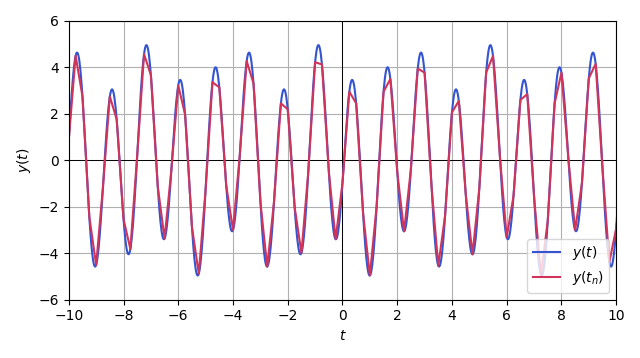
\includegraphics[width=\textwidth]{sources/second/sins dt=0.25 B=4/3_y_cmp(sampling).png}
        \caption{Сравнительный график $y(t)$ и $y(t_n)$}
    \end{minipage}
\end{figure}
Теперь разница между сигналами заметна на сравнительном графике.\newpage
Попробуем восстановить сигнал по сэмплированному образу с тем же значением $B$:
\begin{figure}[H]
    \begin{minipage}{0.49\textwidth}
        \centering 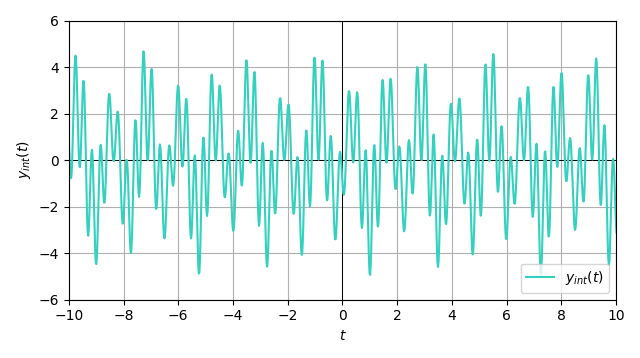
\includegraphics[width=\textwidth]{sources/second/sins dt=0.25 B=4/4_y_interp.png}
        \caption{График восстановленного сигнала $y_{int}(t)$}
    \end{minipage}\hfill
    \begin{minipage}{0.49\textwidth}
        \centering 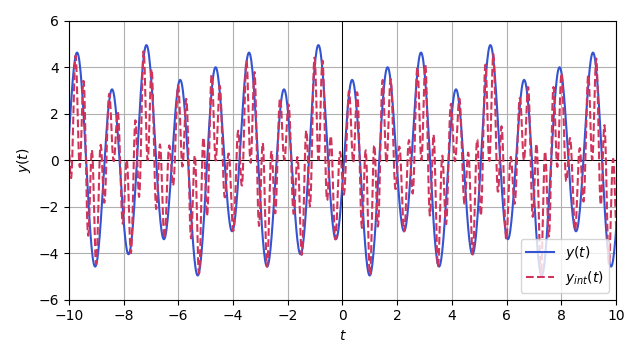
\includegraphics[width=\textwidth]{sources/second/sins dt=0.25 B=4/5_y_cmp(interpolation).png}
        \caption{Сравнительный график $y(t)$ и $y_{int}(t)$}
    \end{minipage}
\end{figure}
Как мы видим, увеличение шага сэмплирования привело к тому, что формула интерполяции не сработала так, как должно --- восстановленный сигнал отличается от исходного.\\[0.5em]
Чтобы это исправить, уменьшим $B$ до $2$ и попробуем ещё раз восстановить сигнал:
\begin{figure}[H]
    \begin{minipage}{0.49\textwidth}
        \centering 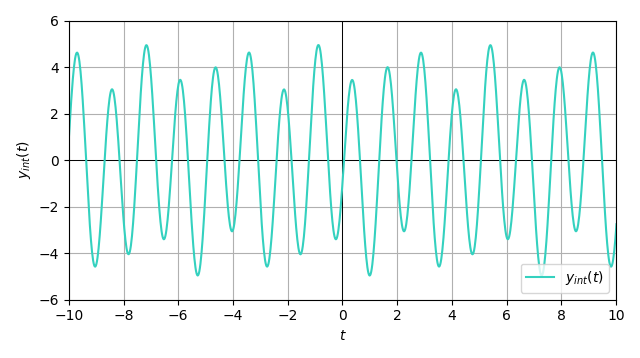
\includegraphics[width=\textwidth]{sources/second/sins dt=0.25 B=2/4_y_interp.png}
        \caption{График восстановленного сигнала $y_{int}(t)$}
    \end{minipage}\hfill
    \begin{minipage}{0.49\textwidth}
        \centering 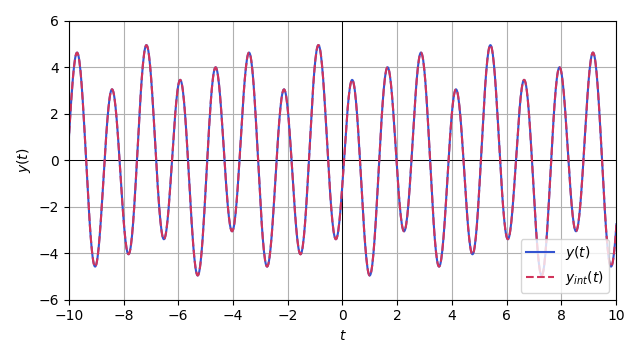
\includegraphics[width=\textwidth]{sources/second/sins dt=0.25 B=2/5_y_cmp(interpolation).png}
        \caption{Сравнительный график $y(t)$ и $y_{int}(t)$}
    \end{minipage}
\end{figure}
Теперь восстановить сигнал из сэмплированного удалось.

\addsubsection{Сэмплирование sinus cardinalis}
Перейдём к сэмплированию и интерполяции кардинального синуса. Сначала зададимся параметром $b = 2$ и функцией:
$$y(t) = \text{sinc}(bt) = \text{sinc}(2t)$$
\begin{figure}[H]
    \begin{minipage}{0.49\textwidth}
        \centering 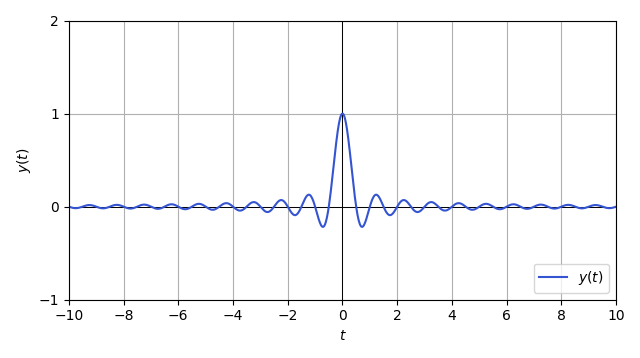
\includegraphics[width=\textwidth]{sources/second/1_sinc_y.png}
        \caption{График $y(t)$}
    \end{minipage}\hfill
    \begin{minipage}{0.49\textwidth}
        \centering 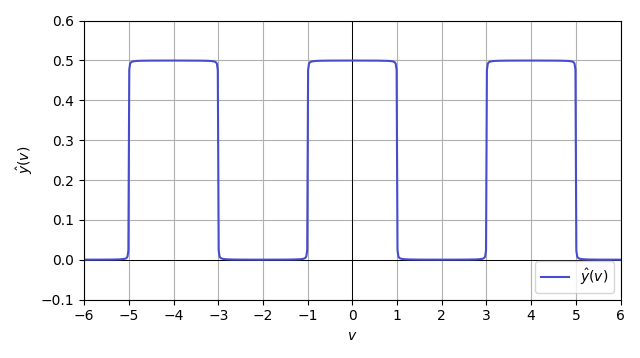
\includegraphics[width=\textwidth]{sources/second/6_sinc_image.png}
        \caption{Фурье-образ $y(t)$}
    \end{minipage}
\end{figure}
Фурье-образ кардинального синуса, как и ожидалось, представляет собой прямоугольную функцию. \newpage
Оставим параметр $B = 2$, а шаг дискретизации установим $\Delta t = \nicefrac{1}{2}$. И вот так будет выглядеть сравнительный график исходного и сэмплированного сигналов:
\begin{figure}[H]
    \centering 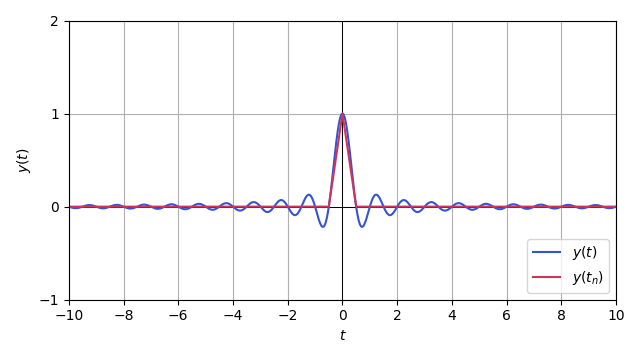
\includegraphics[width=0.49\textwidth]{sources/second/sinc dt=0.5 B=2/3_y_cmp(sampling).png}
    \caption{Сравнительный график $y(t)$ и $y(t_n)$}
\end{figure}
Как мы видим, сэмплированный сигнал сведён к треугольной волне. Теперь попробуем восстановить сигнал:
\begin{figure}[H]
    \begin{minipage}{0.49\textwidth}
        \centering 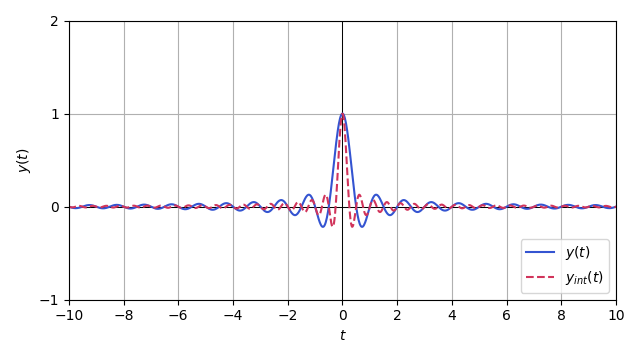
\includegraphics[width=\textwidth]{sources/second/sinc dt=0.5 B=2/5_y_cmp(interpolation).png}
        \caption{Сравнительный график $y(t)$ и $y_{int}(t)$}
    \end{minipage}\hfill
    \begin{minipage}{0.49\textwidth}
        \centering 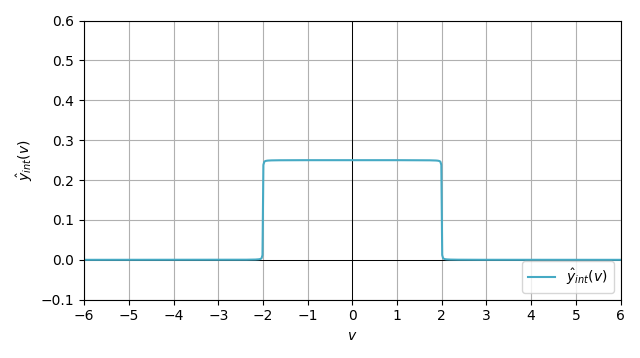
\includegraphics[width=\textwidth]{sources/second/sinc dt=0.5 B=2/7_interp_image.png}
        \caption{Фурье-образ сигнала $y_{int}(t)$}
    \end{minipage}
\end{figure}
Как видим, интерполяция не сработала, и восстановленный сигнал отличается от исходного. Также и Фурье-образ восстановленного сигнала представляет собой прямоугольную функцию другой ширины и амплитуды. Чтобы это исправить, изменим шаг сэмплирования до $\Delta t = \nicefrac{1}{4}$:
\begin{figure}[H]
    \begin{minipage}{0.49\textwidth}
        \centering 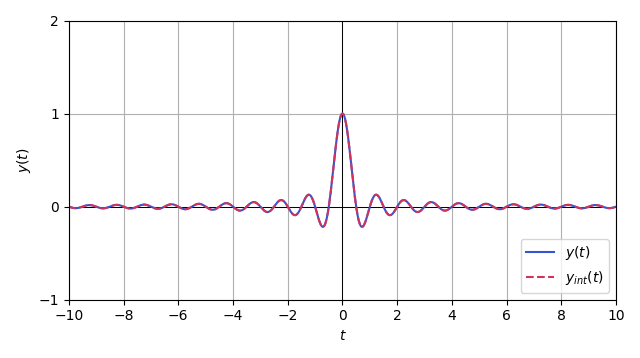
\includegraphics[width=\textwidth]{sources/second/sinc dt=0.25 B=2/5_y_cmp(interpolation).png}
        \caption{Сравнительный график $y(t)$ и $y_{int}(t)$}
    \end{minipage}\hfill
    \begin{minipage}{0.49\textwidth}
        \centering 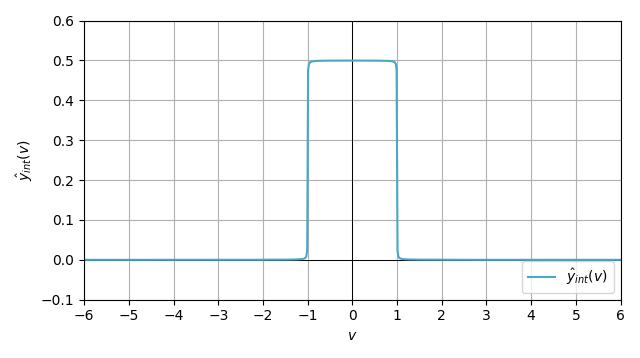
\includegraphics[width=\textwidth]{sources/second/sinc dt=0.25 B=2/7_interp_image.png}
        \caption{Фурье-образ сигнала $y_{int}(t)$}
    \end{minipage}
\end{figure}
Восстановленный сигнал и его Фурье-образ идентичны исходному. Заметим, что прямоугольная волна только одна в образе и образ больше не периодичный.\\[0.5em]
\textbf{Вывод:}
\begin{quotebox}
    Мы исследовали теорему Найквиста-Шеннона-Котельникова на примере двух разных сигналов. Дейсвительно, восстановить исходный сигнал получалось тогда, когда шаг дискретизации $\Delta t$ был меньше $\nicefrac{1}{(2B)}$. При этом образ Фурье восстановленного сигнала не периодичный, в отличие от образа Фурье исходного сигнала.
\end{quotebox}
\end{document}